\section{Training}

\textbf{Loss: cross-entropy with label smoothing.} At every non-padding position, the loss measures how much probability the model gives to the correct next word. With label smoothing {[}17{]}, the target puts weight \(1 - \varepsilon\) on the correct word and spreads \(\varepsilon = 0.1\) evenly over the whole vocabulary. This stops the model from becoming over-confident.

\[\mathcal{L} = -\frac{1}{|S|} \sum_{t \in S} \sum_{w} q_t(w) \log p_t(w), \qquad q_t(w) = (1 - \varepsilon)\,[w = y_{t+1}] + \frac{\varepsilon}{|V|} \tag{3.23}\]

Here \(S\) is the set of non-padding positions, and \([w = y_{t+1}]\) is 1 for the correct word and 0 otherwise. For example, if the model gives the correct word probability 0.6, the plain cross-entropy loss is \(-\ln 0.6 = 0.51\). With probability 0.1 it would be \(2.30\).

\textbf{Two-phase transfer learning.} The encoder starts from Swin-T weights trained on ImageNet {[}10{]}, so it already knows how to see. The decoder starts from random values. Training therefore has two phases (Figure 3.20):

\begin{itemize}
\tightlist
\item
  \textbf{Phase 1 (epochs 1--2).} The encoder is frozen, and only the decoder learns (learning rate \(1.5 \times 10^{-4}\)). This prevents large, random early gradients from damaging the pretrained features.
\item
  \textbf{Phase 2 (epoch 3 onwards).} Everything trains, with a 10 times smaller learning rate for the encoder (\(1.5 \times 10^{-5}\)) than for the decoder (\(1 \times 10^{-4}\)).
\end{itemize}

\begin{figure}
\centering
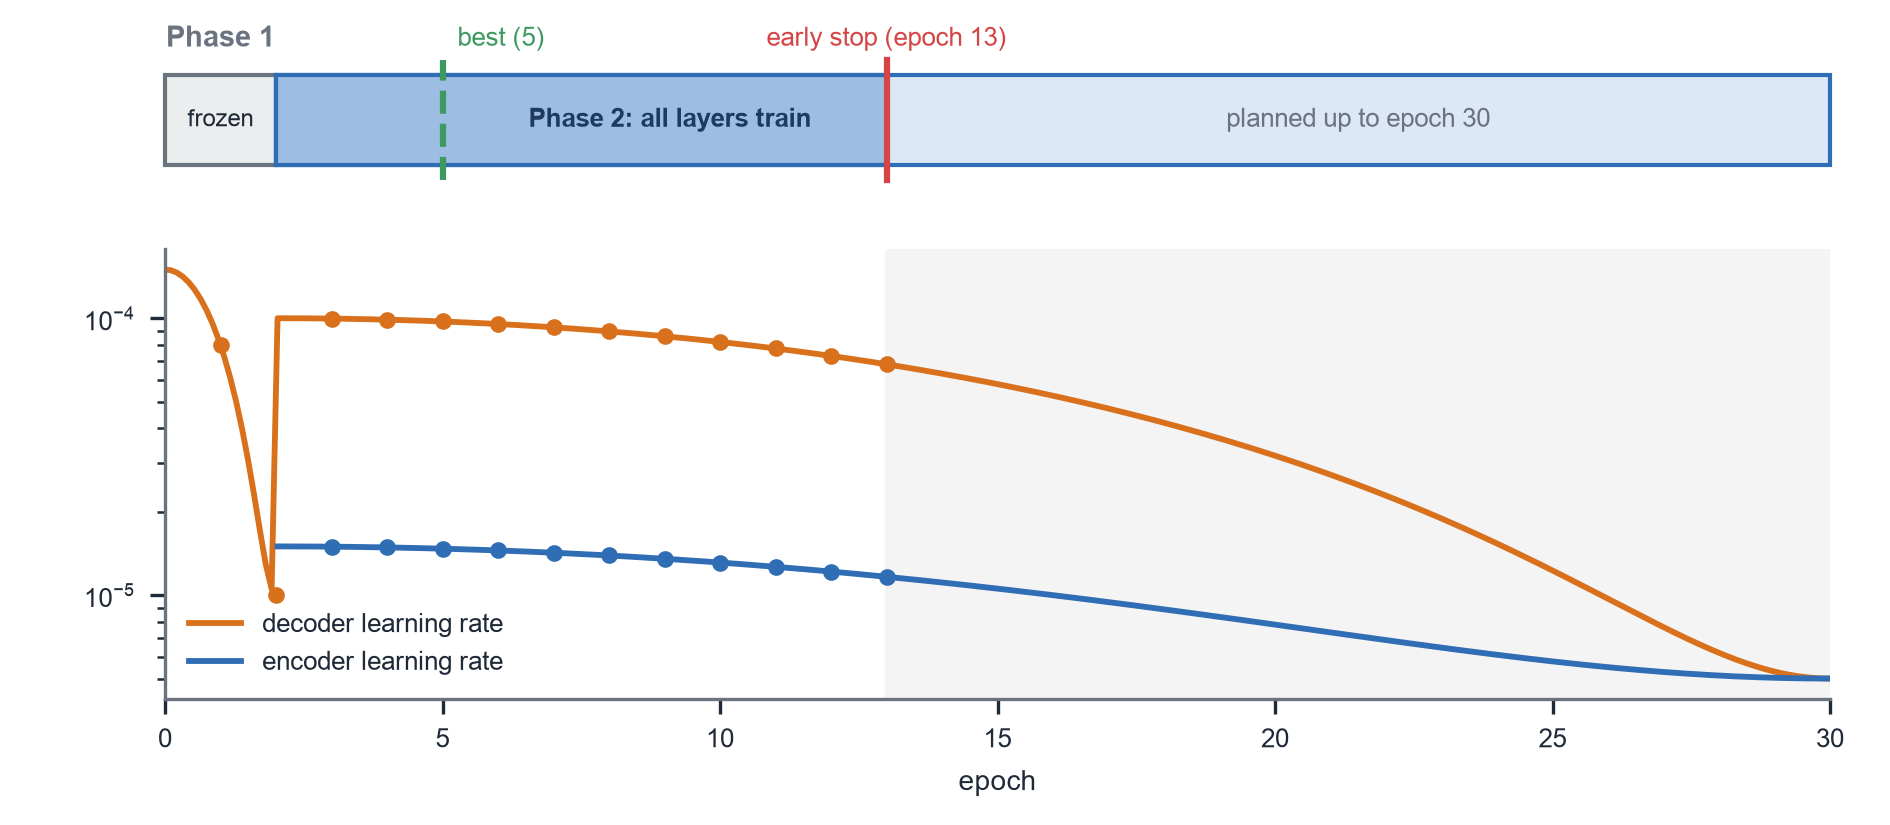
\includegraphics[width=1\linewidth,height=\textheight,keepaspectratio]{figures/fig3_34_two_phase.png}
\caption{Two-phase training. Top: the phase timeline, with the best epoch (5) and the early stop (13). Bottom: the cosine learning-rate schedules of the encoder and decoder; dots are the values logged during our run.}
\end{figure}

\textbf{Optimiser and schedule.}

\begin{itemize}
\tightlist
\item
  \textbf{AdamW {[}18{]}} applies weight decay 0.05 to the weight matrices only, not to biases, LayerNorm parameters, embeddings or the position-bias tables.
\item
  \textbf{Cosine schedule {[}19{]}:} within each phase, the learning rate falls smoothly along a cosine curve after every batch:
\end{itemize}

\[\eta_k = \eta_{\min} + \tfrac{1}{2}\left(\eta_{\max} - \eta_{\min}\right)\left(1 + \cos\frac{\pi k}{K}\right) \tag{3.24}\]

where \(k\) is the current step and \(K\) the number of steps in the phase. At the halfway point of phase 1, for example, the decoder's rate is \(10^{-5} + 0.5 \times 1.4 \times 10^{-4} = 8 \times 10^{-5}\), matching the value logged after epoch 1.

\begin{itemize}
\tightlist
\item
  \textbf{Gradient clipping:} gradients are rescaled whenever their overall size exceeds 1.0.
\item
  \textbf{Early stopping:} training stops after 8 epochs without improvement in validation loss. In our run the best validation loss, 4.556, came at epoch 5, and training stopped after epoch 13 (Chapter 6).
\end{itemize}

\needspace{35\baselineskip}

\begin{longtable}[]{@{}
  >{\raggedright\arraybackslash}p{(\linewidth - 2\tabcolsep) * \real{0.5000}}
  >{\raggedright\arraybackslash}p{(\linewidth - 2\tabcolsep) * \real{0.5000}}@{}}
\caption{Model, training and generation settings.}\tabularnewline
\toprule\noalign{}
\begin{minipage}[b]{\linewidth}\raggedright
Part
\end{minipage} & \begin{minipage}[b]{\linewidth}\raggedright
Setting
\end{minipage} \\
\midrule\noalign{}
\endfirsthead
\toprule\noalign{}
\begin{minipage}[b]{\linewidth}\raggedright
Part
\end{minipage} & \begin{minipage}[b]{\linewidth}\raggedright
Setting
\end{minipage} \\
\midrule\noalign{}
\endhead
\bottomrule\noalign{}
\endlastfoot
Encoder & Swin-T (torchvision, ImageNet-1K weights): patch 4, channels 96--768, depths (2, 2, 6, 2), heads (3, 6, 12, 24), window 7, stochastic depth 0.2 \\
Decoder & 6 layers, width 768, 8 heads, feed-forward 3,072, dropout 0.2, weight tying, sinusoidal positions \\
Data & Images \(224 \times 224\) with flip, rotation, shift and colour jitter; captions of 40 tokens; vocabulary 8,729 (minimum count 5) \\
Optimisation & AdamW, weight decay 0.05, batch 32, phase 1 (2 epochs) learning rate \(1.5 \times 10^{-4}\), phase 2 learning rates \(1.5 \times 10^{-5}\) (encoder) and \(1 \times 10^{-4}\) (decoder), cosine schedule, gradient clipping 1.0, mixed precision \\
Regularisation & Label smoothing 0.1, word dropout 0.1, early stopping (patience 8) \\
Generation & Beam search (\(k = 4\) for evaluation), length penalty 0.7, repetition penalty 1.5, trigram blocking, at most 40 tokens \\
Code & \texttt{caption\_model.py}, \texttt{swin\_model.py}, \texttt{decoder\_model.py}, \texttt{train.py}, \texttt{eval.py} (PyTorch {[}25{]}) \\
\end{longtable}

\needspace{24\baselineskip}

\section{Summary: the four attention types}

\begin{longtable}[]{@{}
  >{\raggedright\arraybackslash}p{(\linewidth - 12\tabcolsep) * \real{0.1429}}
  >{\raggedright\arraybackslash}p{(\linewidth - 12\tabcolsep) * \real{0.1429}}
  >{\raggedright\arraybackslash}p{(\linewidth - 12\tabcolsep) * \real{0.1429}}
  >{\raggedright\arraybackslash}p{(\linewidth - 12\tabcolsep) * \real{0.1429}}
  >{\raggedright\arraybackslash}p{(\linewidth - 12\tabcolsep) * \real{0.1429}}
  >{\raggedright\arraybackslash}p{(\linewidth - 12\tabcolsep) * \real{0.1429}}
  >{\raggedright\arraybackslash}p{(\linewidth - 12\tabcolsep) * \real{0.1429}}@{}}
\caption{The attention types used in the model.}\tabularnewline
\toprule\noalign{}
\begin{minipage}[b]{\linewidth}\raggedright
Type
\end{minipage} & \begin{minipage}[b]{\linewidth}\raggedright
Used in
\end{minipage} & \begin{minipage}[b]{\linewidth}\raggedright
Queries from
\end{minipage} & \begin{minipage}[b]{\linewidth}\raggedright
Keys and values from
\end{minipage} & \begin{minipage}[b]{\linewidth}\raggedright
Extra term
\end{minipage} & \begin{minipage}[b]{\linewidth}\raggedright
Weights per head
\end{minipage} & \begin{minipage}[b]{\linewidth}\raggedright
Purpose
\end{minipage} \\
\midrule\noalign{}
\endfirsthead
\toprule\noalign{}
\begin{minipage}[b]{\linewidth}\raggedright
Type
\end{minipage} & \begin{minipage}[b]{\linewidth}\raggedright
Used in
\end{minipage} & \begin{minipage}[b]{\linewidth}\raggedright
Queries from
\end{minipage} & \begin{minipage}[b]{\linewidth}\raggedright
Keys and values from
\end{minipage} & \begin{minipage}[b]{\linewidth}\raggedright
Extra term
\end{minipage} & \begin{minipage}[b]{\linewidth}\raggedright
Weights per head
\end{minipage} & \begin{minipage}[b]{\linewidth}\raggedright
Purpose
\end{minipage} \\
\midrule\noalign{}
\endhead
\bottomrule\noalign{}
\endlastfoot
Window (W-MSA) & Encoder, 1st block of each pair & Tokens of one window & The same window & Position bias \(B\) & \(49 \times 49\) per window & Local context \\
Shifted window (SW-MSA) & Encoder, 2nd block of each pair & Tokens of a shifted window & The same window & \(B\) + mask \(\Phi\) & \(49 \times 49\) per window & Link neighbouring windows \\
Masked self-attention & Decoder, every layer & Words & Words & Causal mask \(M\) & \(39 \times 39\) & Context of earlier words \\
Cross-attention & Decoder, every layer & Words & Image memory \(Z\) & --- & \(39 \times 49\) & Look at the image \\
\end{longtable}
